\documentclass[fontsize = 10pt, paper= a4,twocolumn,column_gap=5zw]{jlreq}

\usepackage[dvipdfmx]{graphicx}
\usepackage{color}
\usepackage{listings}
\usepackage{url}
\definecolor{OliveGreen}{rgb}{0.0,0.6,0.0}
\definecolor{Magenta}{cmyk}{0, 1, 0, 0}
\definecolor{colFunc}{rgb}{1,0.07,0.54}
\definecolor{CadetBlue}{cmyk}{0.62,0.57,0.23,0}
\definecolor{Brown}{cmyk}{0,0.81,1,0.60}
\definecolor{colID}{rgb}{0.63,0.44,0}
\lstset{
language={C},                   %言語の指定
basicstyle={\ttfamily\small},        %書体の指定
backgroundcolor={\color[gray]{.95}}, %背景色と透過度
keywordstyle={\color{blue}},         %キーワード(int, ifなど)の書体指定
commentstyle={\color{OliveGreen}},   %注釈の書体 
stringstyle=\color{Magenta},         %文字列
frame=single,                        %枠縁(leftline,topline,bottomline,lines,trBL,shadowbox, single)
numbers=left,                        %行番号表示
numberstyle={\ttfamily\small},       %行番号の書体指定
breaklines=true,                     %折り返し(自動改行)
breakindent = 10pt,                  %自動改行後のインデント量(デフォルトでは20[pt])	
tabsize=2,                           %タブの大きさ
captionpos=t                         %キャプションの場所(t,b : "tb"ならば上下両方に記載)
}
\renewcommand{\lstlistingname}{図} % キャプション名の指定

\begin{document}

\title{統計分析法 第6週レポート}
\author{202212022 田島瑞起}
\date{2023/11/21}
\maketitle
\section{設問1}
    A,Bについてのヒストグラムを下記の図で示す。
    \begin{figure}
        \centering
        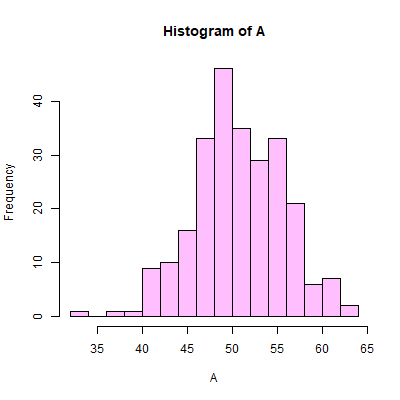
\includegraphics[width=4cm]{6-1.png}
    \end{figure}
    \begin{figure}
        \centering
        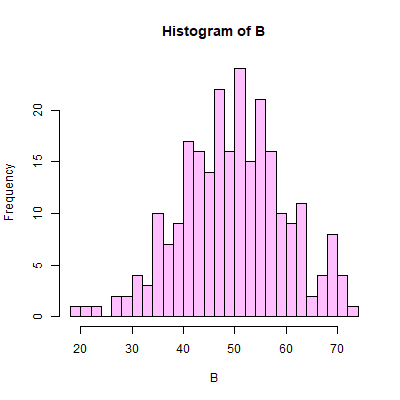
\includegraphics[width=4cm]{6-2.png}
    \end{figure}
\section{設問2}
    A群のデータ平均値がB群のデータ平均値よりも大きいことを示すために,
    AとBを統合したデータから10,000回のサンプリングを実行し,サンプリングしたデータを二分割し,
    平均値の差をとり,平均値の分布上で実測値がどれほどの確率で起こっているか確かめ,その後有意水準を満たしているか確認する。
    この方法でpを算出した結果,p=0.0656となり,Aの平均値はBの平均値よりも大きいという帰無仮説が支持されることが分かった。
    また,理想分布及び実測値は下の図で示す。
    \begin{figure}
        \centering
        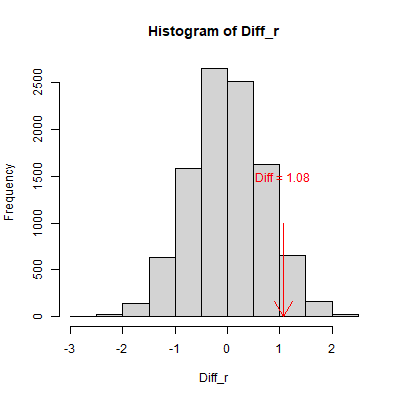
\includegraphics[width=4cm]{6-3.png}
    \end{figure}
\section{設問3}
    設問2で使用したコードを編集して,n=50におけるpの平均値は13.086標準偏差は0.0365と算出された。
    次にnの値を50~50000まで変化させたときpの平均値及び標準偏差がどのように推移するか確認する。
    nの値の間隔は5000とし実行した結果が下記の図になる。
    \begin{figure}
        \centering
        
\includegraphics[width=4cm]{6-4.png}
    \end{figure}
    \begin{figure}
        \centering
        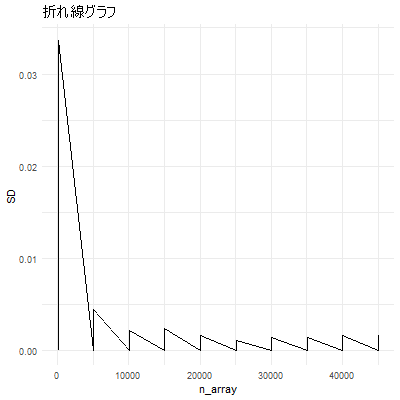
\includegraphics[width=4cm]{6-5.png}
    \end{figure}
    今回の課題では計算量を考慮した結果nのサンプリング間隔が大きくなってしまったため,正確な値は不明であるがn=5000あたりから結果が安定しているため,その付近の値でサンプリングすれば良いと考えられる。


\section{設問4}
    permを利用して検定したところ,p=0.06709と算出され,これは優位水準を満たす値なので,AのデータのほうがBのデータよりも大きいことが分かる。
    t-testでは,pは有意水準を満たしており,2つのデータに差は無いと結論できる。
    今課題で個人的に考えたのは,ランダマイゼーションは,2群を混ぜてからサンプリングすることによって,偏りを減らすことにより,2群の差異をt-testよりもシビアに判定することが出来るのではないかと考えた。

\section{ソースコード}
\begin{lstlisting}[basicstyle=\ttfamily\footnotesize, frame=single, caption=s2212022-1.c ,label=s2212022-1.c]
    #課題1
ReadData <- read.table('data_r.txt')
A <- ReadData$V1
B <- ReadData$V2
A <- A[2:length(A)]
B <- B[2:length(B)]
A <- as.numeric(A)
B <- as.numeric(B)
png("6-1.png", width = 400, height = 400)
hist(A,breaks=20,col='#ff00ff40')
dev.off()
png("6-2.png", width = 400, height = 400)
hist(B,breaks=20,col='#ff00ff40')
dev.off()
#課題2
Diff <- mean(A) - mean(B)
n <- 9999
Diff_r <- numeric(n+1)
Data <- c(A,B)
for(i in 1:n){
    data_r <- sample(Data,replace=F)
    A_r <- data_r[1:length(A)]
    B_r <- data_r[(length(A)+1):length(data_r)]
    Diff_r[i] <- (mean(A_r) - mean(B_r))
}
Diff_r[n+1] <- Diff
p <- sum(Diff_r >= Diff)(n+1)

png("6-3.png",width=400,height=400)
hist(Diff_r)
arrows(x0 = Diff,  y0 = 0, x1 = Diff, y1 = 1000, col = "red", code = 1, angle = 30)
text(Diff,1500,labels = paste("Diff =", round(Diff, 2)), col = "red")
dev.off()

#課題3
n <- 49
p_array <- numeric(10)
for(j in 1:10){
    for(i in 1:n){
        data_r <- sample(Data,replace=F)
        A_r <- data_r[1:length(A)]
        B_r <- data_r[(length(A)+1):length(data_r)]
        Diff_r[i] <- (mean(A_r) - mean(B_r))
    }
    Diff_r[n+1] <- Diff
    p <- sum(Diff_r >= Diff)/(n+1)
    p
    p_array[j] <- p
}
mean(p_array)
sd(p_array)

n_array <- seq(50,50000,5000)
mean_array <- numeric(length(n_array))
sd_array <- numeric(length(n_array)) 
for(k in n_array){
    n <- k
    p_array <- numeric(10)
    for(j in 1:10){
        for(i in 1:n){
            data_r <- sample(Data,replace=F)
            A_r <- data_r[1:length(A)]
            B_r <- data_r[(length(A)+1):length(data_r)]
            Diff_r[i] <- (mean(A_r) - mean(B_r))
        }
        Diff_r[n+1] <- Diff
        p <- sum(Diff_r >= Diff)/(n+1)
        p_array[j] <- p
    }
    mean_array <- append(mean_array,mean(p_array))
    sd_array <- append(sd_array,sd(p_array))
}

install.packages("ggplot2")
# ライブラリの読み込み
library(ggplot2)
# グラフの作成
df <- data.frame(n = n_array, mean = mean_array, sd = sd_array)
# 折れ線グラフの描画
png("6-4.png",width=400,height=400)
ggplot(df, aes(x = n, y = mean)) +
  geom_line() +
  labs(title = "折れ線グラフ",
       x = "n_array",
       y = "Mean") +
  theme_minimal()

dev.off()

png("6-5.png",width=400,height=400)
ggplot(df, aes(x = n, y = sd)) +
  geom_line() +
  labs(title = "折れ線グラフ",
       x = "n_array",
       y = "SD") +
  theme_minimal()
dev.off()

#課題4

# permパッケージをインストールして読み込む
install.packages("perm")
library(perm)
# permTS()関数を使用して順位和検定を実行
perm_test_result <- permTS(A, B, alternative = "greater")

# 結果の表示
print(perm_test_result)

# t検定を実行
t_test_result <- t.test(A, B, alternative = "greater")

# 結果の表示
print(t_test_result)
    \end{lstlisting}

\end{document}